%%%%%%%%%%%%%%%%%%%%%%%%%%%%%%%%%%%%%%%%%%%%%%%%%%%%%%%%%%%%%%%%
% Sim
%%%%%%%%%%%%%%%%%%%%%%%%%%%%%%%%%%%%%%%%%%%%%%%%%%%%%%%%%%%%%%%%
\section{仿真}

% ////////////////////////////////////////
\subsection{被控对象建模}
可以用上一节中推导出的式\eqref{eqModelTotal}建立被控对象微分方程,
若忽略火星自转的影响,
也可以建立向量形式的微分方程
\begin{equation}
    \ddot{\vec{r}} = \frac{\mu}{||\vec{r}||^3}\vec{r}+\vec{L}+\vec{D} \label{eqSimF3}
\end{equation}
其中阻力向量为
\begin{align}
    \vec{D} = -D\frac{\vec{v}}{||\vec{v}||} \label{eqSimF1}
\end{align}
升力向量$\vec{L}$与铅垂面夹角为倾侧角$\sigma$,
为了能将$\vec{L}$用其他已知向量表示,
需要构造一对与$\vec{L}$同平面的正交单位向量。
已知$\vec{v}$与$\vec{r}$张成铅垂面,
另构造一个垂直于铅垂面且在惯性系中方向向上的单位向量$\vec{n}_2$,
和另一个与$\vec{r}$同方向的单位向量$\vec{n}_1$,
则$\vec{n}_1$位于铅垂面内,
此时$\vec{L}$与$\vec{n}_1$的夹角即为倾侧角,
$\vec{n}_1$和$\vec{n}_2$即为用于表示$\vec{L}$的正交单位向量,
即
\begin{align}
    \vec{n}_2 =& \frac{\vec{r}\times\vec{v}}{||\vec{r}\times\vec{v}||} \notag\\
    \vec{L}=\vec{n}_1\cos\sigma + \vec{n}_2\sin\sigma \label{eqSimF2}
\end{align}
微分方程式\eqref{eqSimF3}\eqref{eqSimF1}\eqref{eqSimF2}共同组成被控对象模型。
建立飞行器被控对象模型的模块框图如图\ref{figSimPlant}所示。
\begin{center}
	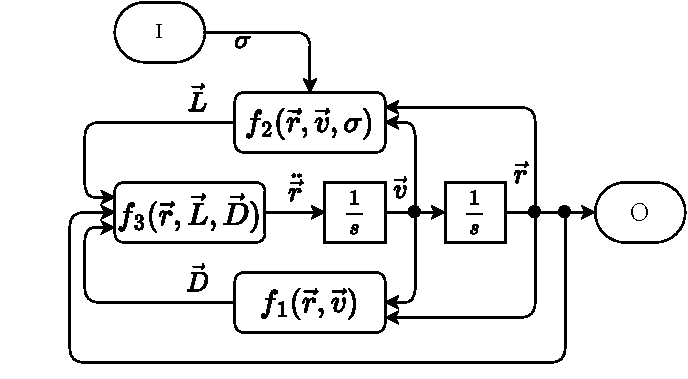
\includegraphics[scale=0.8]{plant.pdf}  \\
	\figcaption{被控对象模型的模块框图}\label{figSimPlant}
\end{center}
图中,被控对象的输入(控制量)为倾侧角$\sigma$,
输出为位置$\vec{r}$。
图中的3个多输入单输出函数分别为式\eqref{eqSimF1Total}\eqref{eqSimF2Total}\eqref{eqSimF3Total}
\begin{align}
    \left\{\begin{aligned}
    h =& ||\vec{r}||-R \\
    \rho =& \rho_0e^{-h/h_s} \\
    D =& \frac{1}{2}\rho||\vec{v}||^2S_{\text{ref}}C_D \\
    \vec{D} =& f_1(\vec{r},\vec{v}) = -D\frac{\vec{v}}{||\vec{v}||}
\end{aligned}\right. \label{eqSimF1Total}
\end{align}
\begin{align}
    \left\{\begin{aligned}
    h =& ||\vec{r}||-R \\
    \rho =& \rho_0e^{-h/h_s} \\
    L =& \frac{1}{2}\rho||\vec{v}||^2S_{\text{ref}}C_L \\
    \vec{n}_2 =& \frac{\vec{r}\times\vec{v}}{||\vec{r}\times\vec{v}||} \\
    \vec{n}_1 =& \frac{\vec{r}}{||\vec{r}||} \\
    \vec{L} =& f_2(\vec{r},\vec{v},\sigma) = L(\vec{n}_1\cos\sigma + \vec{n}_2\sin\sigma)
\end{aligned}\right. \label{eqSimF2Total}
\end{align}
\begin{equation}
    \ddot{\vec{r}} = f_3(\vec{r},\vec{L},\vec{D}) = \frac{\mu}{||\vec{r}||^3}\vec{r}+\vec{L}+\vec{D} \label{eqSimF3Total}
\end{equation}
式中$R$为火星半径。

% ////////////////////////////////////////
\subsection{直通模块与端点模块}

